\chapter{Probability and Statistics}

\section{Probability Distributions}
References: 
\begin{itemize}
	\item Lista, Statistical Methods for Data Analysis in Particle Physics, Second Edition, ISBN: 978-3-319-62840-0.
	\item Hughes, Hase, Measurements and their Uncertainties, ISBN: 978-0-19-956633-4.
\end{itemize}

\subsection{Chi-Squared Distribution}
A $\chi^2$ random variable with n degrees of freedom is the sum of $n$ standard normal variables. The normalized probability distribution of a $\chi^2$ variable is given by:
\begin{align}
	f(\chi^2;n)=\dfrac{(\chi^2)^{n/2-1}e^{-\chi^2/2}}{2^{n/2}\Gamma(n/2)}.
	\label{eq:chi-square}
\end{align}
$\Gamma$ is the so-called \textit{gamma function}, the analytical extension of the fatorial. The expected value of a $\chi^2$ distribution is equal to the number of degrees of freedom $n$ and the variance is equal to $2n$. $\chi^2$ distributions are shown in the following figure for different number of degrees of freedom $n$.

\begin{figure}
    \centering
    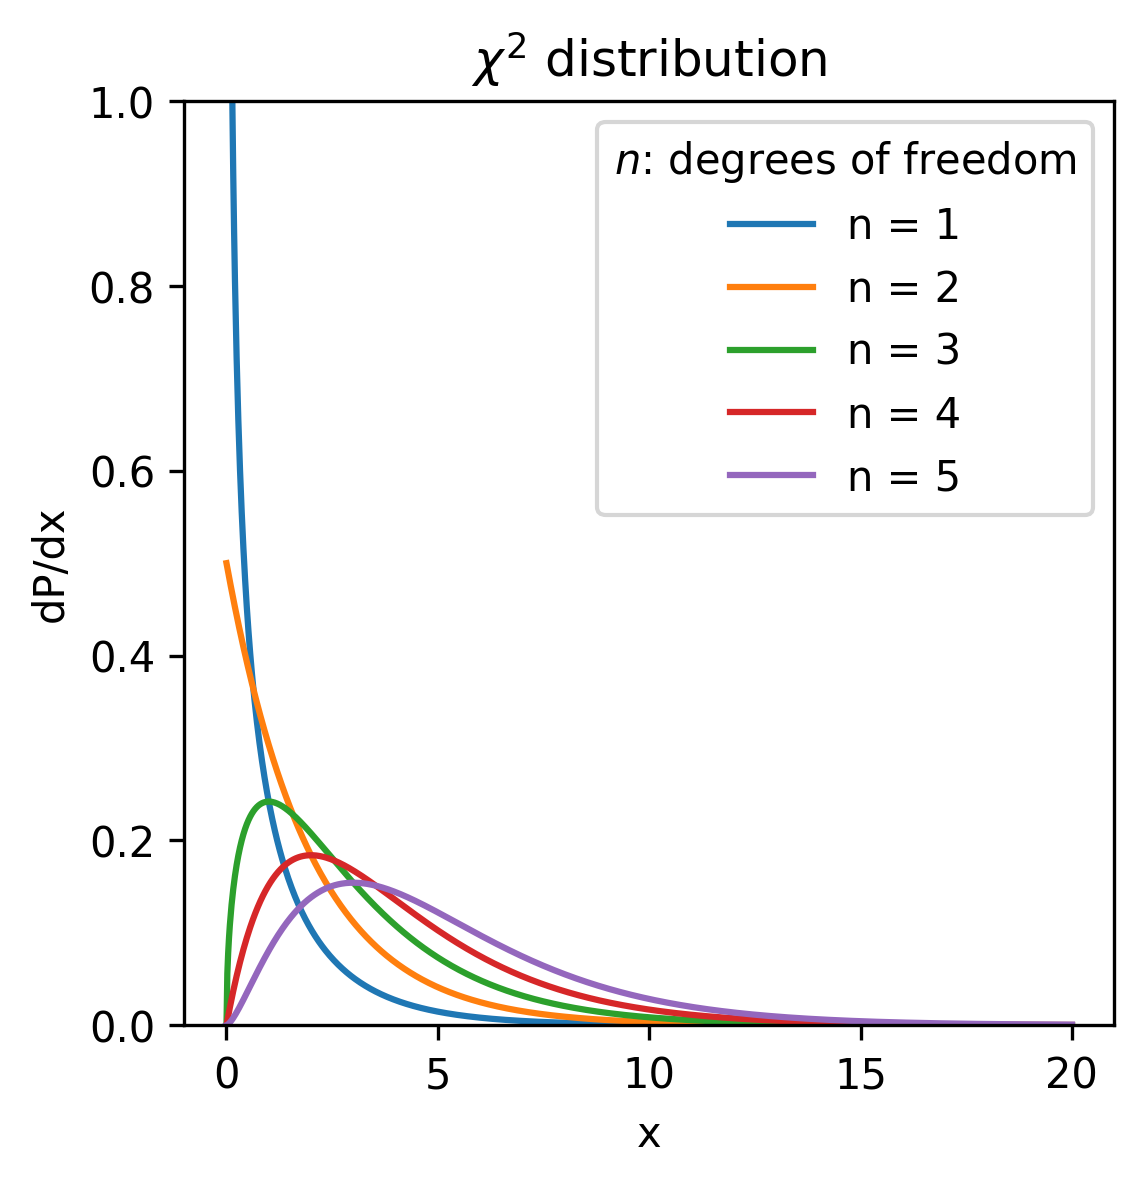
\includegraphics[width=0.6\linewidth]{media/prob-stats/chi-square-distribution.png}
    \caption{Chi-square distribution for different number of degrees of freedom $n$.}
    \label{fig:chi-square-distribution}
\end{figure}

For $n=2$, the $\chi^2$ distribution is a special case of the gamma distribution and is identical to an exponential distribution with the mean $\mu=n=2$ and variance of $\sigma^2=2n=4$. The cumulative probability function, $P(\chi^2;n)$:
\begin{align}
	P(\chi^2_{min} \leq \chi^2 \leq \infty; n) = \int_{\chi^2_\mathrm{min}}^{\infty} f(\chi^2;n) \, d\chi^2 
	\label{eq:chi-square-cdf}
\end{align}
gives the probability that were the sample distribution drawn from the hypothesized parent distribution, one would obtain a value $\chi^2$ equal to, or greater than, $\chi^2_\mathrm{min}$. 

\subsubsection{Using $\chi^2$ as a hypothesis test}
Equation \ref{eq:chi-square} and \ref{eq:chi-square-cdf} can be used to perform hypothesis test. We expect that if the proposed model is in good aggrement with the data, $\chi^2_\mathrm{min}$ will be close to the \textit{mean} of the $\chi^2$ distribution and so $\chi^2_\mathrm{min} \approx n$. For many degrees of freedom, the $\chi^2$ distribution becomes more symmetric and the median, mode, and mean become similar and we would expect for a good match between sample and parent distributions with a corresponding probability $P(\chi^2_\mathrm{min} \approx n;n) \approx 0.5$. We learn about the quality of the aggreement between sample and parent by analyzing $P(\chi^2_\mathrm{min};n)$, the probabaility of obtaining the observed value, or higher, of $\chi^2_\mathrm{min}$ for a given number of degrees of freedom. If the value of $\chi^2_\mathrm{min}$ is significantly greater than $n$, the probability $P(\chi^2_\mathrm{min} > n;n)$ is small \textbf{(show figure here)}. Under such circumstances, there are discrepancies between the model and the data which are unlikely to be explained by random statistical fluctuations in the sample distrubution. This could arise from either (i) an incorrect null hypothesis\footnote{The null hypothesis is that the sample distribution is well modeled by a proposed parent distribution and that any scatter between the two distributions is a result of random statistical variations in the sample.}, or (ii) an incorrect evaluation or assumption about the uncertainties. Conversely, if the value of $\chi^2_\mathrm{min}$ is less than $n$, the cumulative probability distribution function, $P(\chi^2_\mathrm{min};n)$, becomes greater than $0.5$ and tends towards unity. This is not an indication of an improved fit, but rather suggests that the standard errors used in the determination of the $\chi^2$ statistic have been overestimated, resulting in an unrealistically small value of $\chi^2$. 

We now turn to the question of when to reject the hypothesis on the grounds of the value of $\chi^2_\mathrm{min}$ being too large to attribute to statistical fluctuations in the data set. Obviously, there is not one critical value of $P(\chi^2_\mathrm{min};n)$ which determines whether the hypothesis is rejected; in this treatment we will investigate the evolution of $P(\chi^2_\mathrm{min};n)$ as a function of the results being two or three standard deviations away from the mean. In stastics texts, the $5\%$ level of significance is often chosen as the critical value; i.e. if $P(\chi^2;n)\leq0.05$ the hypothesis is said "to be rejected at the 5\% level". As with the sampling of any probability distribution function, the most probable value returned will be the expected expected value or mean. However, it could also be within two standard deviations of the mean \textbf{[cite Hughes and Hase]}. For a test of a particular null hypothesis, we would therefore expect to obtain a value of $\chi^2 \approx n$ but would not be surprised to find $\chi^2$ within two standard deviations of the mean, i.e. in the range $n - 2\sqrt{2n} \leq \chi^2_\mathrm{min}\leq n + 2\sqrt{2n}$. The probability of obtaining a value of $n + 2\sqrt{2n}$ or higher is approximately $4\times10^{-2}$. Due to the asymmetry of $\chi^2$ distribution, this probability has a very weak dependence on $n$; for five degrees of freedom, the probability derived from Equation \ref{eq:chi-square-cdf} is $P(11.3;5) = 0.045$; for $n=20$, $P(32.6;20)=0.037$ and for $n=100$, $P(128;100)=0.029$. The probability of finding a value of $\chi^2_\mathrm{min}$ greater than three standard deviations from the mean, i.e. $\chi^2_\mathrm{min}>n+2\sqrt{n}$ is an order of magnitude smaller and is approximately $5\times10^{-3}$.

Although the probability of finding a value of $\chi^2_\mathrm{min}$ greater than $n+3\sigma$ is rather low, $P(n+3\sigma;n)\approx10^{-3}$, genuinely incorrect models will give significantly lower probabilities, say $P(\chi^2_\mathrm{min};n)\approx10^{-18}$. It is for the experimenter to decide at which  threshild the null hypothesis is rejected. Although firs can be accepted at the $P(\chi^2_\mathrm{min};n)\approx10^{-3}$ level, it is not advisable to do this as a matter of course. It would be a better strategy to find the origin of the discrepancy between the model and data.

\begin{itemize}
	\item For a reasonable fit, the value of $P(\chi^2;n)\approx0.5$.
	\item If $P(\chi^2_\mathrm{min};n)\rightarrow1$, check your calculations for the uncertainties in the measurements.
	\item The null hypothesis is generally not rejected if the value of $\chi^2\mathrm{min}$ is within $\pm 2\sigma$ of the mean.
	\item The null hypothesis is questioned if $P(\chi^2_\mathrm{min};n)\approx10^{-3}$ or $P(\chi^2_\mathrm{min};n)>0.5$.
	\item The null hypothesis is rejected if $P(\chi^2_\mathrm{min};n)<10^{-4}$.
\end{itemize}

\paragraph{The reduced $\chi^2$ statistic:} In order to ascertain whether a particular null hypothesis should be rejected at a particular confidence level, the probabilities of obtaining the observed value of $\chi^2_\mathrm{min}$ or higher given the number of degrees of freedom must be calculated using Equation \ref{eq:chi-square-cdf}. However, we can obtain a quick indication as to whether the nulll hypothesis should be rejected by considering the so-called reduced chi-squared statistic, $\chi^2_\nu$, which is simply the value of $\chi^2$ divided by the number of degrees of freedom:
\begin{align}
	\chi^2_\nu = \dfrac{\chi^2_\mathrm{min}}{n}.
\end{align} 

A good match between the sample and parent distribution occurs when $\chi^2_\nu \approx 1$. We can understand why the null hypothesis is not rejected if $\chi^2 \approx 1$ by considering that for good agreement between the sample and parent distribution each point will differ from its expected value, i.e. the mean, by typically the standard deviation of the mean (standard error). Thus, each term in the summation of the $\chi^2$ statistic should be of order one, with the result that $\chi^2\approx N$. Typically, as the number of degrees of freedom is similar to the number of data points, $\chi^2_\nu$ is thus expected to be unity. If the value of $\chi^2_\nu$ is much larger than one, it is likely that the null hypothesis should be rejected. A very small value of $\chi^2$ is also unlikely -- either the error bars have been overestimated, which reduces the value of $\chi^2$, or the observed and expected values are unrealistically close. Again, it is for the experimenter to decide at which confidence the null hypothesis should be rejected in terms of the reduced chi-squared statistic. Earlier, we discussed how one would not be surprised if the observed value of $\chi^2$ was within $2 \sigma$ of the mean for a good fit, and that the null hypothesis should only be questioned if the value of $\chi^2_\mathrm{min}$ was larger than, say, $3\sigma$ from the mean. As the standard deviation of the $\chi^2$ distribution depends on $n$, the confidence intervals for $\chi^2$ also depend on $n$. Recall that for a Gaussian distribution the $n+1\sigma$, $n+2 \sigma$, and $n+3 \sigma$ intervals correspond to the $68\%$, $95\%$, and $99.7\%$ confidence limits. The $3\sigma$ confidence limit of $\chi^2$ is tabulated for several values of $n$ in Table \ref{tab:reduced-chi-squared-3sigma}.

\begin{itemize}
	\item For a reasonable fit, the value of $\chi^2\approx1$.
	\\item If $\chi^2_\nu \ll 1$, check your calculations for uncertainties in the measurements.
	\item The null hypothesis is questioned if $\chi^2_\nu > 2$ for $n\approx10$.
	\item The null hypothesis is questioned if $\chi^2_\nu > 1.5$ if $n$ is in the approximate range $50\leq n \leq 100$.
\end{itemize}

Although easier to calculate, $\chi^2_\nu$ does not contain as much information as using $\chi^2_\mathrm{min}$ and $\nu$ to calculate $P(\chi^2_\mathrm{min};n)$ \textbf{[cite Hughes and Hase]}. 

\begin{table}
	\centering
	\begin{tabular}{cc}
		\toprule
		$n$ & ($\chi^2_n + 3\sigma$)\\
		\midrule
		5 & 2.9 \\
		10 & 2.3 \\
		20 & 1.9 \\
		30 & 1.8 \\
		50 & 1.6 \\				
		100 & 1.4 \\
		500 & 1.2 \\				
		\bottomrule
	\end{tabular}	
	\caption{Example values of the largest acceptable values of $\chi^2_\nu$ obtained from the ($\chi^2 + 3\sigma$) confidence level for different degrees of freedom, $n$.}
	\label{tab:reduced-chi-squared-3sigma}
\end{table}

\subsubsection{Testing the quality of fit using $\chi^2$}
Consider a number $n$ of measurements ($y_1 \pm \sigma_1, \dots, y_n\pm\sigma_n$), and each measurement $y_i\pm\sigma_i$ corresponds to a value $x_i$ of a variable $x$. Assume we have a model for the dependence of $y$ on the variable $x$ given by a function $f$:
\begin{align}
	y=f(x;\vec{\theta}),
\end{align}
where $\vec{\theta}={\theta_1, \dots, \theta_m}$ is a set of unknown parameters. If the measurements $y_i$ are distributed around the value $f(x_i, \vec{\theta})$ according to a Gaussian distribution with standard deviation equal to $\sigma_i$, the likelihood function for this problem can be written as the product of $n$ Gaussian PDFs:
\begin{align}
	L(\vec{y};\vec{\theta})=\Pi_{i=1}^n \dfrac{1}{\sqrt{2\pi\sigma_i^2}} exp\left[- \dfrac{(y_i-f(x_i;\vec{\theta}))^2}{2\sigma_i^2}\right],
\end{align}
where the notation $\vec{y}={y_1, \dots, y_n}$.

Maximizing $L(\vec{y}, \vec{\theta})$ is squivalent to minimize $-2logL(\vec{y}, \vec{\theta})$:
\begin{align}
	 -2logL(\vec{y}; \vec{\theta}) = \sum_{i=1}^{n} \dfrac{\left(y_i - f(x_i;\vec{\theta})\right)^2}{\sigma_i^2} + \sum_{i=1}^{n}log2\pi\sigma_i^2.
\end{align}
The last term does not depend on the parameters $\theta$ if the uncertainties $\sigma_i$ are known and fixed, hence it is a constant that can be dropped when performing the minimization. The first term to be minimized is a $\chi^2$ variable:
\begin{align}
	\chi^2(\vec{\theta}) = \sum_{i=1}^{n}\dfrac{\left( y_i - f(x_i; \vec{\theta}) \right)^2}{\sigma_i}.
\end{align}

The terms: 
\begin{align}
	r_i=y_i-\hat{y}_i = y_i - f(x_i;\hat{\vec{\theta}}),
\end{align}
evaluated at the fit values $\hat{\vec{\theta}}$ of the parameters $\vec{\theta}$, are called *residuals*. An example of the fit performed on a computer-generated dataset with the minimum $\chi^2$ method is shown in the following figure. 

\begin{figure}
    \centering
    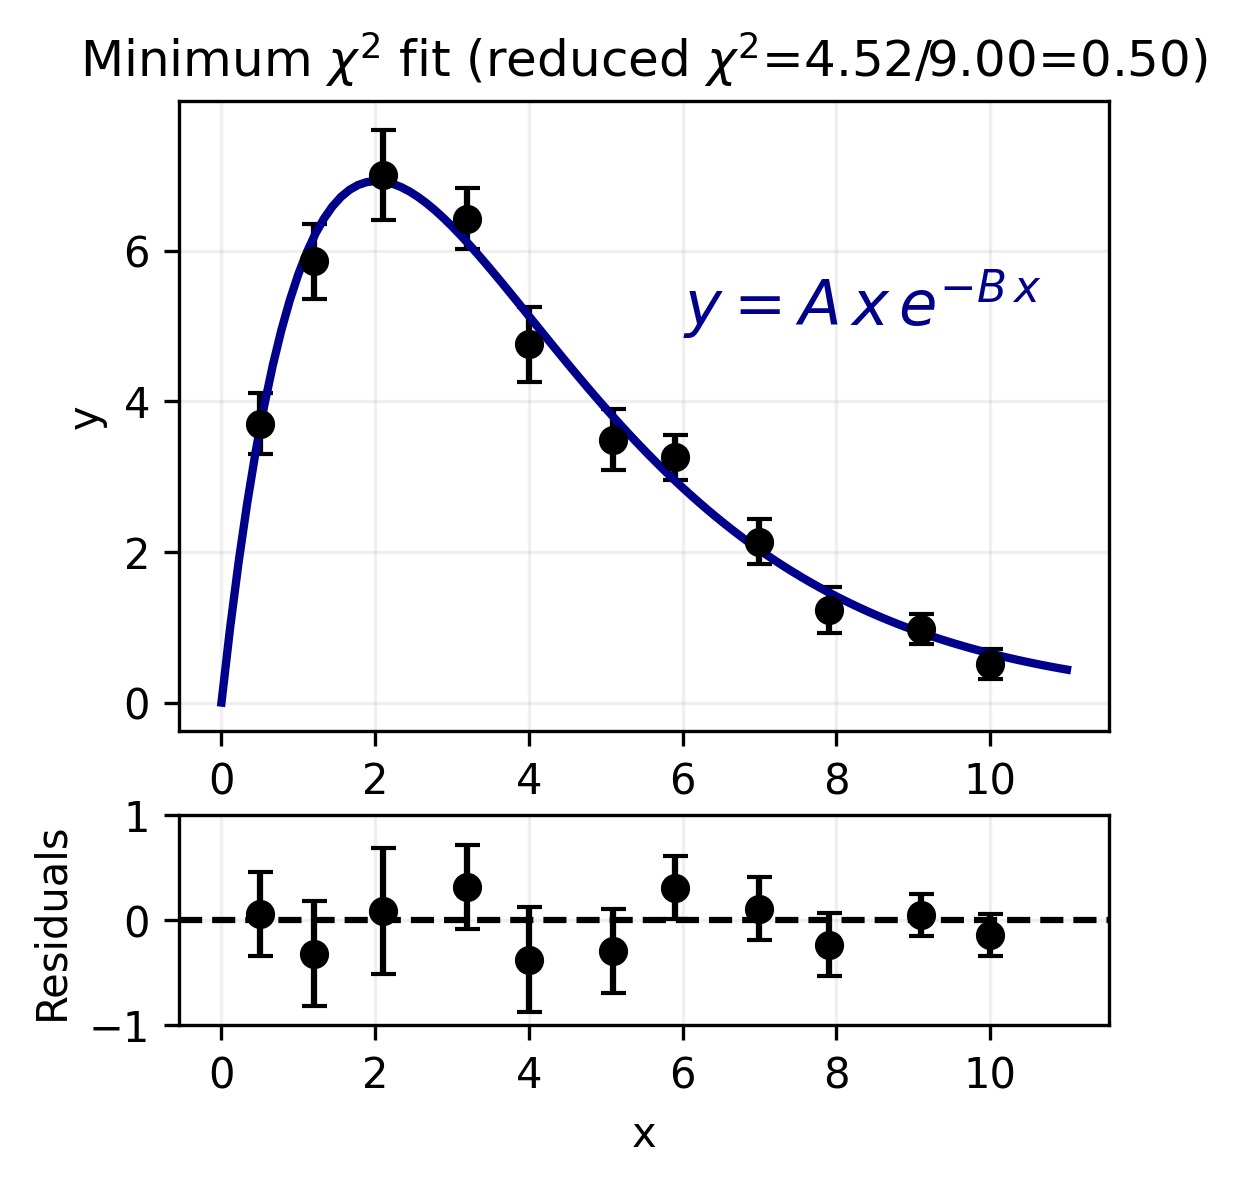
\includegraphics[width=0.6\linewidth]{media/prob-stats/minimum-chi-square-fit.png}
    \caption{Minimum $\chi^2$ fit of a function model to a set of data points with error bars.}
    \label{fig:minimum-chi-square-fit}
\end{figure}

Here, the points with the error bars are used to fit a function model of the type $y=f(x)=Axe^{-Bx}$, where $A$ and $B$ are unknown parameters determined by the fit. The fit curve is superimposed as solid blue line. Residuals are shown in the bottom section of the plot. Reduced chi-square $\chi_\nu^2=\chi^2/ndf$ is a goodness-of-fit statistic calculated by dividing the chi-squared values by the degrees of freedom. It assess how well a model fits data as follows:
\begin{itemize}
	\item $\chi^2_\nu \approx 1$: the fit is good; the model accurately describes the data,
	\item $\chi^2_\nu>1$: poor fit; the model is not sufficient, or experimental errors are underestimated,
	\item $\chi^2<1$: over-fitting; the model is too complex, or errors are overestimated.
\end{itemize}

\section{Hypothesis Testing}
\subsection{Discovery thresholds and upper limits}
\section{Confidence Intervals}
\subsection{Feldman-Cousins Method}
\section{Errors and uncertainties}
\section{Bayesian and frwquentist statistics}


